\chapter{Introduction}

This chapter is based on Munson Chapter 1.
\section{Definitions}
\subsection{Fluid}
A fluid is a substance that \textbf{deforms continuously} under any \textbf{shear stress}\footnote{A shear stress $\tau$ is the tangential component of a force that acts on an surface}. Equivalently we can say: A fluid is a material that cannot statically resist a shear stress. It needs to move in order to resist a shear stress.

The resistance of a fluid to shear stress is determined by viscosity

\subsection{Basic Laws of Physics}
The basic laws of physics that a fluid dynamics problem must satisfy are:
\begin{enumerate}
    \item conservation of mass
    \item Newton's 2nd law  ("conservation of momentum")
    \item conservation of energy (first law of thermodynamics)
    \item 2nd law of thermodynamics
\end{enumerate}

\subsection{Properties of a fluid}
\begin{itemize}
    \item \textbf{density} $\rho=\frac mV,\qquad [\rho]=\frac {\operatorname{kg}}{\operatorname{m}^3}$
    \item \textbf{specific volume} $v=\frac Vm=\rho^{-1}\qquad [v]  =\frac {\operatorname{m}^3}{\operatorname{kg}}$
    \item \textbf{specific weight} $\gamma=\rho g\qquad [\gamma]=\frac{\operatorname{kg}\operatorname{m}}{\operatorname{m}^3\operatorname{s}^2}=\frac{\operatorname{N}}{\operatorname{m}^3}$
    \item \textbf{specific gravity} $SG=\frac{\rho}{\rho_{H_2O}}$
\end{itemize}
\subsection{Normal Conditions}
% Context?
% From Thermodynamics: $rho = f(T,p)$\footnote{This is only applicable if we are not in a two-phase region.}
Normal conditions are at athmospheric pressure ($1atm$) at $300K$. At these conditions:
\begin{itemize}
    \item $\rho_{H_2O} = 1000 \mathrm{kg/m^3}$
    \item $\rho_{Air} = 1.22 \mathrm{kg/m^3} \approx \frac{\rho_{H_2O}}{1000}$
\end{itemize}

\subsection{Ideal Gas Law}
$$
\rho = \frac{p}{RT}
$$
where $p$ is the \textbf{absolute pressure} (pressure relative to vacuume), $T$ is the \textbf{absolute temperature} (in $\mathrm{K}$), $\rho$ is the \textbf{density} and $R$ is the \textbf{specific gas constant} (sometimes denoted as $R_s$).

\subsection{Viscosity}
To quantify the response of a fluid to a shear stress, we need to have a measure of how quickly a fluid moves.

\subsubsection{No Slip Condition, Shear Strain Rate}
\begin{center}
\shadowbox{At a solid boundary a fluid will have zero velocity relative to the boundary.}
\end{center}
\begin{figure}[H]
    \begin{center}
    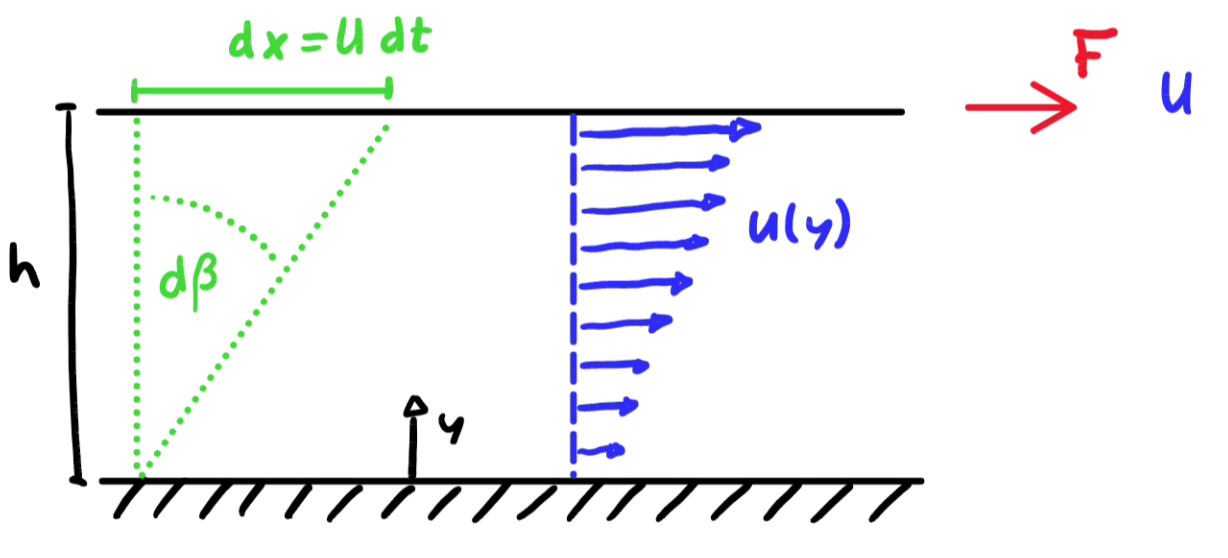
\includegraphics[width=0.4\textwidth]{NoSlip.png}
    \caption{Two plates have a fluid in between. After applying a pure shear force, the top plate moves with velocity $U$. This moves our magically marked atoms on the top by $dx=Udt$.}
    \end{center}
\end{figure}
We can pose the tangent of $d\beta$ to find the deplacement at a height $h$. For small deplacements we can find the change in angle over time to be the \textbf{shear strain rate} $\dot \gamma$
$$
\tan d\beta = \frac {dx}h \approx d\beta \qquad d\beta << 1\implies \frac {d\beta}{dt} = \frac{dx}{hdt}=\frac Uh =: \dot \gamma\qquad [\dot \gamma] = s^{-1}
$$
\paragraph{Notes}
Anywhere in the domain, we can approximate that
$$
\frac Uh \approx\frac {dU}{dy}
$$
\subsection{Newtonian Fluids}
How can we relate the equations of shear stress and shear strain rate? 
We define as \textbf{newtonian fluids} as all the fluids, where the relationship between the applied shear stress is proportional to the shear strain rate (i.e. how much does it respond):
\begin{equation}
\tau = \frac FA \propto \frac {dU}{dy}\implies \tau = \mu \frac{dU}{dy}\label{eq:newtonian_fl}
\end{equation}

\shadowbox{For a newtonian fluid, the more force I apply, the faster it moves (linearly).}
\subsection{Viscosity}

\subsubsection{Dynamic Viscosity}
We define the factor of linearity $\mu$ in \ref{eq:newtonian_fl} to be \textbf{viscosity} (often called dynamic viscosity)
$$
[\mu] = \frac {\mathrm{kg}}{\mathrm m\cdot \mathrm s}
$$

\subsubsection{Kinematic Viscosity}

$$
\nu := \frac \mu \rho\qquad [\nu] =\frac {\mathrm m^2}{s} 
$$
\subsubsection{Notes} 
\begin{itemize}
    \item The stress-strain rate relation in general can be more complex in other flow geometries. But for newtonian fluids it remains linear.
    \item In theory, viscosity $\mu$ is tensor of rank 4. Through symetries, this often collapses to a scalar.
    \item In solids, there are so called Hookean materials which are analogous to Newtonian fluids, where the strain is linear whereas in newtonians the strain rate is linear.
\end{itemize}
\subsubsection{Common Values of Viscosity}
At normal conditions:
\begin{figure}[H]
    \begin{minipage}{0.45\textwidth}
        \centering
        \begin{tabular}{ll}
        \textbf{Material} & \textbf{Viscosity $\mu$ in $\mathrm{kg}/(\mathrm m\cdot \mathrm s)$}\\
        \hline
        Air      & $1.8\cdot 10^{-5}$                         \\
        \hline
        Water    & $1.1\cdot 10^{-3}$                          \\
        \hline
        "Oil"    & $0.4$                       
        \end{tabular}

    \end{minipage}
    \hfill
    \begin{minipage}{0.45\textwidth}
        \centering
        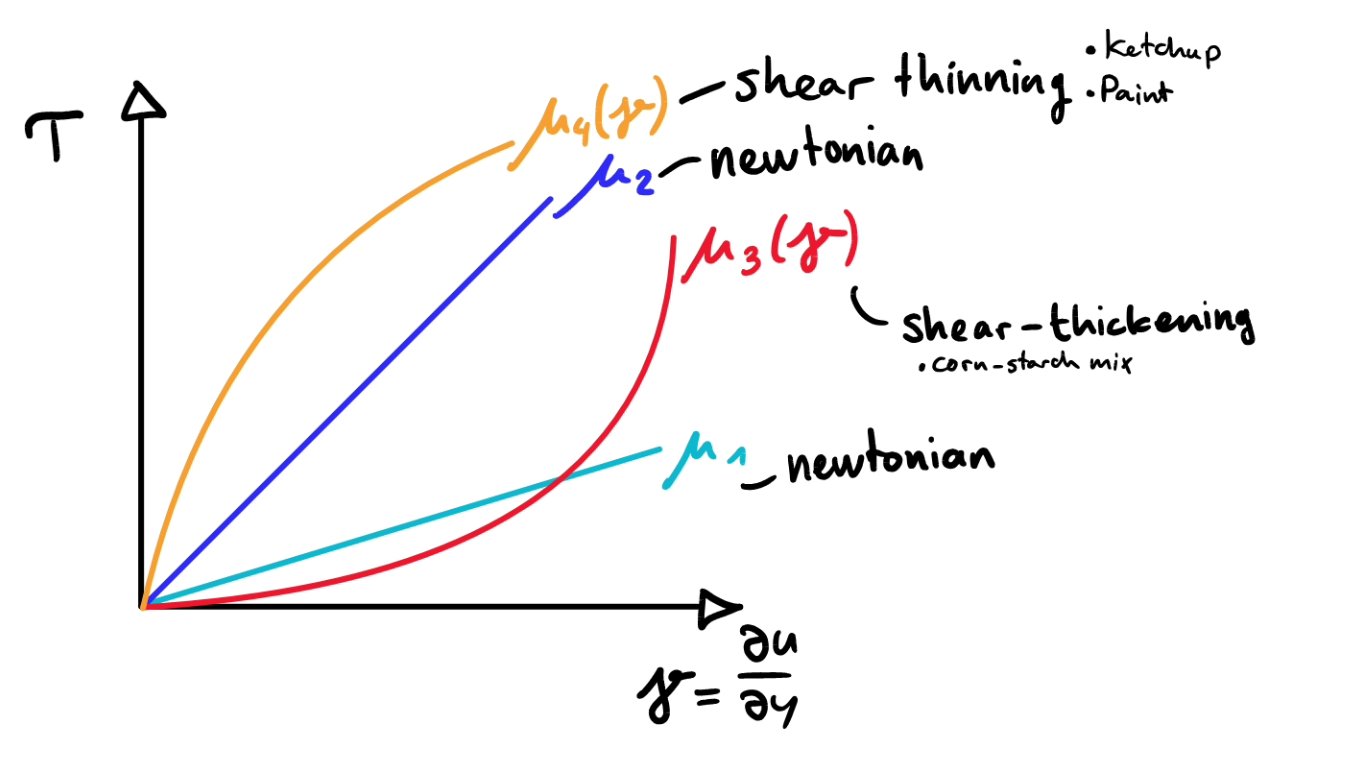
\includegraphics[width=\textwidth]{Newtonian_NonNewtonian.png}

    \end{minipage}
\end{figure}

\paragraph{cgs: Poise}
The poise (only centi-poise is really used) is a commonly used unit for viscosity
$$
\frac{\mathrm g}{\mathrm{cm}\cdot\mathrm s} =: \mathrm{poise} = \mathrm p = 100 \mathrm{cp}
$$

\section{Application: Simple Flow Problem (Munson 1.69)}
We consider the setup in the figure bellow. Two fluids are seperated by an infinite plate at a given height. The top most plate moves at a given velocity $U$. We want to determine the velocity $V$ of the center plate. Additionally we assume that $\mu_2=2\mu_1$.

\begin{figure}[H]
    \begin{minipage}{0.45\textwidth}   
                \centering
            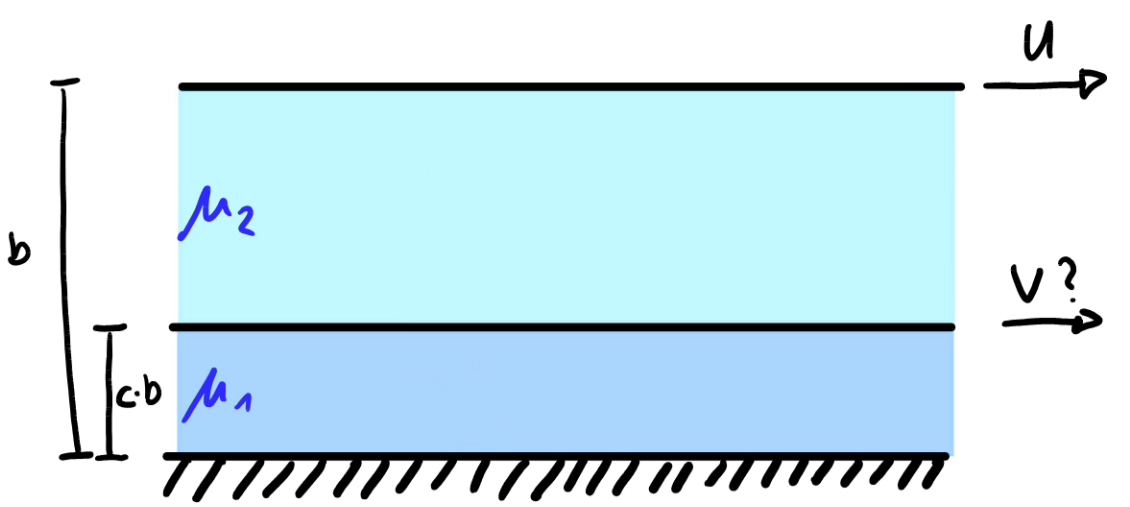
\includegraphics[width=\textwidth]{FlowProblem_1_69a.png}
            \caption{The two fluids with their respective viscosities. The ground plate is fixed and the top moves at a given velocity.}            
    \end{minipage}
    \hfill
    \begin{minipage}{0.45\textwidth}
        \centering
        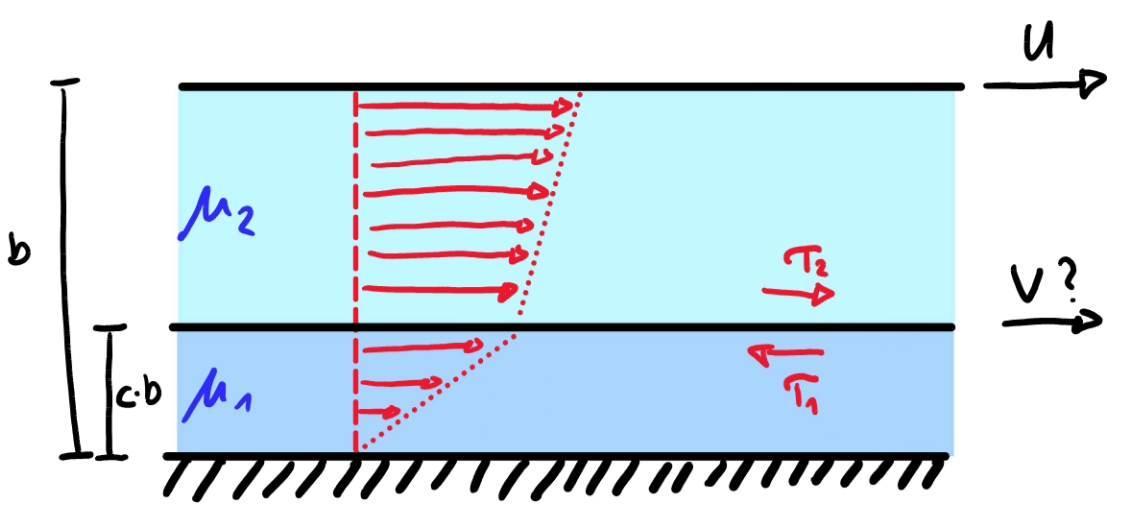
\includegraphics[width=\textwidth]{FlowProblem_1_69b.png}
        \caption{We add shear stresses to the drawing and draw the displacement distribution along the height.}
    \end{minipage}
\end{figure}

We apply the force balance on the middle plate:
\begin{equation*}
    \begin{split}
    \sum F_H = \tau_2A-\tau_1A &\stackrel{*}{=} 0\qquad *: a= 0\\
    \implies \tau_1 &= \tau_2
    \end{split}
\end{equation*}
Expressing $\tau_1$ in terms of variables yields:
$$
\tau_1 = \mu_1\frac V{cb}\stackrel{!}{=}\tau_2=\mu_2\frac{U-V}{(1-c)b}
$$
After solving for $V$ to get:
$$
V=\frac {2c}{1+c}U
$$
To verify boundary conditions, we test for $c=0$ and $c=1$:
$$
\begin{cases}
c=0\implies V=0\\
c=1 \implies V = U
\end{cases}
$$
These results make sense to us.